\documentclass{article}
\usepackage[utf8]{inputenc}
\usepackage{tikz}
\usepackage{amsmath}
\usepackage{ifthen}
\usepackage{amssymb}
\usepackage[top=4cm,bottom=3cm,left=3cm,right=3cm]{geometry}
\usetikzlibrary{automata}
\newboolean{sol}
\newboolean{ex}


%%%% Config here

% Show excercises
\setboolean{ex}{true}
% Show solutions
\setboolean{sol}{true}
%%%

\usepackage{float}
\newcommand{\aufgaben}[2]{
\ifthenelse{\boolean{ex}}{
\ifthenelse{\boolean{sol}}{
	\subsection{Aufgaben}
}{}}{}
\ifthenelse{\boolean{ex}}{#1}{}
\ifthenelse{\boolean{ex}}{
\ifthenelse{\boolean{sol}}{
	\subsection{Lösungen}
}{}}{}
\ifthenelse{\boolean{sol}}{#2}{}
}

\newcommand{\N}{\ensuremath{\mathbb{N}}}
\newcommand{\M}{\ensuremath{\mathcal{M}}}
\newcommand{\classP}{\ensuremath{\mathcal{P}}}
\newcommand{\classNP}{\ensuremath{\mathcal{NP}}}
\newcommand{\co}{\ensuremath{\mathsf{co\text{-}}}}
\newcommand{\pot}{\ensuremath{\mathcal{P}}}
\newcommand{\abs}[1]{\ensuremath{\left\vert #1 \right\vert}}
\newcommand{\menge}[2]{\ensuremath{\left\lbrace #1 \,\middle\vert\, #2 \right\rbrace}}
\newcommand{\ducttape}[1]{\vspace{#1}}
\newcommand{\neglit}[1]{\overline{#1\vphantom{x^a}}}
\newcommand{\recipe}{\raisebox{-.3cm}{
\includegraphics[scale=.15]{images/chefs-cap.png}}\hspace{0.2cm}}
\newcommand{\opt}[1]{\ensuremath{\text{OPT}(#1)}}
\newcommand{\A}[1]{\ensuremath{\mathcal{A}(#1)}}

\begin{document}
\ifthenelse{\boolean{ex}}{
	\ifthenelse{\boolean{sol}}{
		\title{Übungsaufgaben mit Lösung}
	}{
		\title{Übungsaufgaben}
	}
}{
	\ifthenelse{\boolean{sol}}{
		\title{Lösungen}
	}{
		\title{Leeres Blatt}
	}
}
\author{Simon Stroh und Moritz von Looz \\
Fixes von Sebastian Ullrich}
\maketitle
\section{Endliche Automaten}
\aufgaben{
 Gegeben sei folgender nichtdeterministischer endlicher Automat:
\begin{center}
\begin{figure}[H]
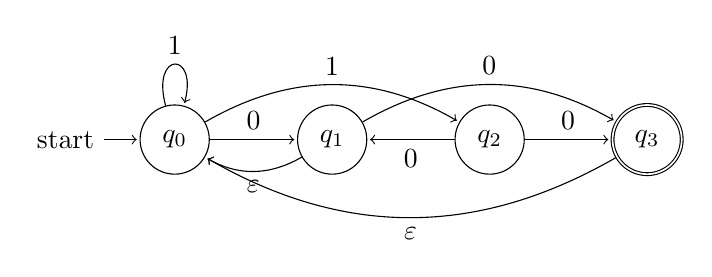
\begin{tikzpicture}[node distance=2cm,shorten >=1pt,auto]
\node[state,initial] 	(q_0)			{$q_0$};
\node[state]		(q_1)	[right of=q_0]	{$q_1$};
\node[state]		(q_2)	[right of=q_1]	{$q_2$};
\node[state,accepting]	(q_3)	[right of=q_2]	{$q_3$};
\path[->]		(q_0)	edge 			node	{$0$}		(q_1)
				edge [bend left]	node	{$1$}		(q_2)
				edge [loop above]	node	{$1$}		()
			(q_1)	edge [bend left]	node	{$\varepsilon$}	(q_0)
				edge [bend left]	node	{$0$}		(q_3)
			(q_2)	edge 			node	{$0$}		(q_1)
				edge			node	{$0$}		(q_3)
			(q_3)	edge [bend left]	node	{$\varepsilon$}	(q_0);
\end{tikzpicture}
\end{figure}
\end{center}
\begin{enumerate}
\item Bilde einen äquivalenten, minimalen DEA.
\item Was sind die Äquivalenzklassen für diesen Automaten bezüglich der Nerode-Relation?
\item Bilde einen regulären Ausdruck, der die gleiche Sprache darstellt wie der Automat.
\item Folgt aus $L$ regulär, dass $L^R$ regulär ist? (Dabei ist $L^R$ die Menge der Wörter in $L$ rückwärtsgeschrieben)
\end{enumerate}
}{%ab hier lösungen.
\begin{enumerate}
\item 
\begin{enumerate}
\item Entferne $\varepsilon$ Übergänge:
\begin{center}
\begin{figure}[H]
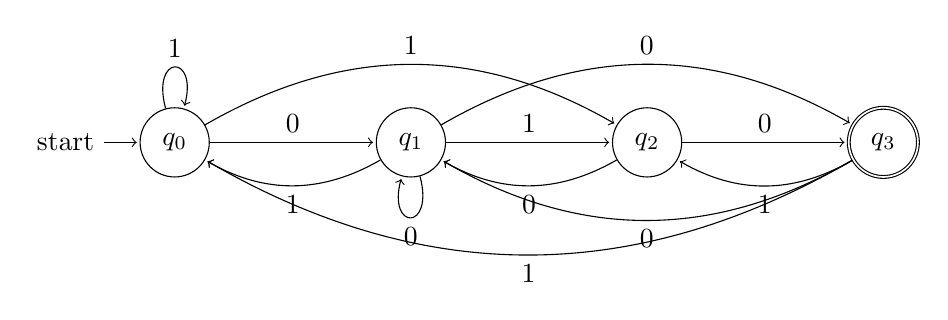
\begin{tikzpicture}[node distance=3cm,shorten >=1pt,auto]
\node[state,initial] 	(q_0)			{$q_0$};
\node[state]		(q_1)	[right of=q_0]	{$q_1$};
\node[state]		(q_2)	[right of=q_1]	{$q_2$};
\node[state,accepting]	(q_3)	[right of=q_2]	{$q_3$};
\path[->]		(q_0)	edge 			node	{$0$}		(q_1)
				edge [bend left]	node	{$1$}		(q_2)
				edge [loop above]	node	{$1$}		()
			(q_1)	edge [bend left]	node	{$1$}		(q_0)
				edge [loop below]	node	{$0$}		()
				edge [bend left]	node	{$0$}		(q_3)
				edge 			node	{$1$}		(q_2)
			(q_2)	edge [bend left]	node	{$0$}		(q_1)
				edge			node	{$0$}		(q_3)
			(q_3)	edge [bend left]	node	{$1$}		(q_0)
				edge [bend left]	node	{$1$}		(q_2)
				edge [bend left]	node	{$0$}		(q_1);
\end{tikzpicture}
\end{figure}
\end{center}

\item Potenzmengenkonstruktion
\begin{figure}[H]
\begin{center}
\begin{tabular}{l l | l | l}
 & & 0 & 1 \\
\hline
$q_0'$:&\{$q_0$\} & \{$q_1$\} & \{$q_0, q_2$\} \\
$q_1'$:& \{$q_1$\} & \{$q_1, q_3$\} & \{$q_0, q_2$\} \\
$q_2'$:& \{$q_0, q_2$\} & \{$q_1, q_3$\} & \{$q_0, q_2$\} \\
$q_3'$:& \{$q_1, q_3$\} & \{$q_0, q_1, q_2, q_3$\} & \{$q_0, q_2$\} \\
$q_4'$:& \{$q_0, q_1, q_2, q_3$\} & \{$q_0, q_1, q_2, q_3$\} & \{$q_0, q_2$\} \\

\end{tabular}
\end{center}
\end{figure}
\item Automat bisher (nach Umbennenung der Zustände):
\begin{figure}[H]
\begin{center}
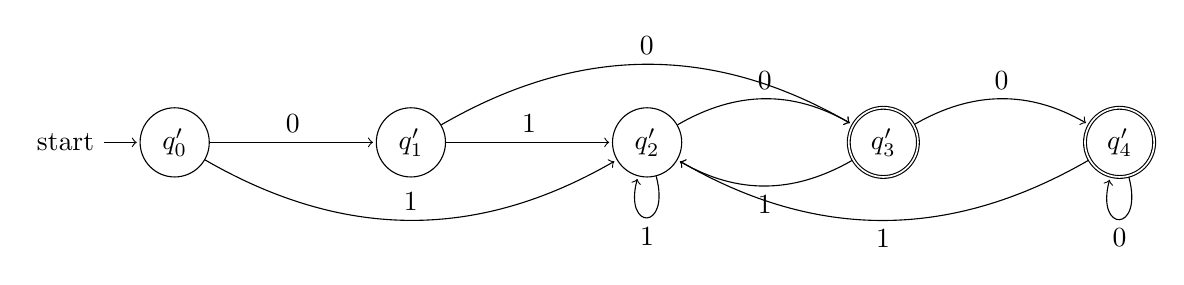
\begin{tikzpicture}[node distance=3cm,shorten >=1pt,auto]
\node[state,initial] 	(q_0)			{$q_0'$};
\node[state]		(q_1)	[right of=q_0]	{$q_1'$};
\node[state] 	  	(q_2)	[right of=q_1]	{$q_2'$};
\node[state,accepting]	(q_3)	[right of=q_2]	{$q_3'$};
\node[state,accepting]	(q_4)	[right of=q_3]	{$q_4'$};
\path[->]		(q_0)	edge 			node	{$0$}		(q_1)
				edge [bend right]	node	{$1$}		(q_2)
			(q_1)	edge [bend left]	node	{$0$}		(q_3)
				edge 			node	{$1$}		(q_2)
			(q_2)	edge [bend left]	node	{$0$}		(q_3)
				edge [loop below]	node	{$1$}		(q_2)
			(q_3)	edge [bend left]	node	{$0$}		(q_4)
				edge [bend left]	node	{$1$}		(q_2)
			(q_4)	edge [loop below]	node	{$0$}		(q_4)
				edge [bend left]	node	{$1$}		(q_2);
\end{tikzpicture}
\end{center}
\end{figure}
\item Minimierung
\begin{enumerate}
\item Trennung durch $\varepsilon$: \{$q_0', q_1', q_2'$\} \{$q_3', q_4'$\}
\item Trennung durch $1$: \{$q_0', q_1', q_2'$\} \{$q_3', q_4'$\}
\item Trennung durch $0$: \{$q_0'$\} \{$q_1', q_2'$\} \{$q_3', q_4'$\}
\item Keine weitere Trennung durch längere Zeugen: Abbruch
\end{enumerate}
\item Minimierter DEA:
\begin{figure}[H]
\begin{center}
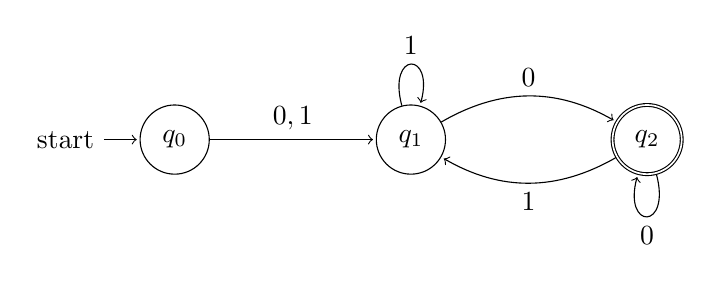
\begin{tikzpicture}[node distance=3cm,shorten >=1pt,auto]
\node[state,initial] 	(q_0)			{$q_0$};
\node[state]		(q_1)	[right of=q_0]	{$q_1$};
\node[state,accepting]	(q_2)	[right of=q_1]	{$q_2$};
\path[->]		(q_0)	edge 			node	{$0,1$}		(q_1)
			(q_1)	edge [loop above]	node	{$1$}		()
				edge [bend left]	node	{$0$}		(q_2)
			(q_2)	edge [bend left]	node	{$1$}		(q_1)
				edge [loop below]	node	{$0$}		();
\end{tikzpicture}
\end{center}
\end{figure}
\end{enumerate}
\item Nach 1. gibt es 3 Klassen. Finde also lediglich Repräsentanten. Etwa:
\begin{enumerate}
\item $[\varepsilon] = \{\varepsilon\}$
\item $[0] = \{0,1\}(\{\varepsilon\} \cup \{0,1\}^*\{1\})$
\item $[00] = \{0,1\}\{0,1\}^*\{0\}$
\end{enumerate}
\item $(0 \cup 1)(0 \cup 1)^*0$ erfüllt die Bedingung
\item Ja, Beweis etwa über strukturelle Induktion über den regulären Ausdruck.
\end{enumerate}
}
\section{Pumping Lemma}
\aufgaben{
Zeige oder widerlege die Regularität folgender Sprachen:
\begin{enumerate}
\item $\{a^ib^j | i \leq j\}$
\item $\{w | w\mbox{ enthält nicht die Zeichenkette } abc \mbox{ oder }cba\}$
\item $\{a^ib^j | i \geq j\}$
\item $\{www | w \in \Sigma^* \}$
\item $\{w | w\mbox{ enthält nicht genau zweimal }a\}$
\item $\{w | w\mbox{ ist kein Palindrom }\}$
\item Sei $\Sigma = \{0,1,+,=\}$ und $L = \{x=y+z | x,y,z \mbox{ sind Binärzahlen und }x = y + z\}$
\end{enumerate}
}{
\begin{enumerate}
\item Widerlege mithilfe des Pumping Lemmas.
\item Die Sprache ist regulär: Konstruktion eines NEA der die Sprache, die die Zeichenketten $abc$ oder $cba$ enthält ist trivial. Das Komplement ist also regulär.
\item Mithilfe der ersten Sprache. Wäre $\{a^ib^j | i \geq j\}$ regulär, könnte man den dazugehörigen Automaten umbauen zu einem, der das Komplement erkennt. 
Damit ist ein Automat zu $\{a^ib^j | i \leq j\}$ leicht zu konstruieren.
\item Widerlege mit Pumping Lemma
\item Beweis ähnlich wie die zweite Sprache: Ein Akzeptor zum Komplement ist einfach zu konstruieren, damit ist das Komplement regulär und auch diese Sprache.
\item Argumentiere wieder über das Komplement und das Pumping Lemma
\item Widerlege mit Pumping Lemma
\end{enumerate}
}
\section{Turingmaschinen und Entscheidbarkeit}
\aufgaben{
\begin{enumerate}
\item Wieviele verschiedene Sprachen gibt es? Wie steht das im Verhältnis zu der Anzahl der Turingmaschinen? Kann man dadurch eine Aussage über die Existenz von nichtentscheidbaren Sprachen machen?
\item Schreibe jeweils eine Turingmaschine, die die folgenden Sprachen erkennt:
\begin{enumerate}
\item $\menge{a^ib^i}{i \in \N_0}$
\item $\{a^ib^j\ | i \leq j\}$
\item $\{w | w\mbox{ enthält nicht die Zeichenkette } abc \mbox{ oder }cba\}$
\item Sei $\Sigma = \{0,1,+,=\}$ und $L = \{x=y+z | x,y,z \}$
\end{enumerate}
\item Zeige, dass eine Sprache entscheidbar ist gdw. eine Turingmaschine existiert, die bei Eingabe eines Wortes der Sprache das nächste Wort nach \textit{shortlex}-Ordnung (primär nach Länge, sekundär lexikographisch geordnet) ausgibt.
\item Zeige, dass eine Sprache semientscheidbar ist gdw. eine Turingmaschine und eine Wohlordnung (Ordnung mit kleinstem Element) existieren, sodass die TM bei Eingabe eines Wortes der Sprache das nächste Wort der Sprache bezüglich dieser Ordnung ausgibt.
\item Formuliere das Problem der Entscheidung, ob ein endlicher Automat und ein regulärer Ausdruck äquivalent sind, als Sprache und zeige, dass diese Sprache entscheidbar ist.
\item Finde eine Lösung für folgendes PCP: $\{(ab,abab),(b,a),(aba,b),(aa,a)\}$
\item Zeige, dass eine TM, die auf den Teil des Bandes, auf dem die Eingabe, steht nicht schreiben kann, nur reguläre Sprachen erkennen kann.
\end{enumerate}
}{
\begin{enumerate}
 \item Es gibt überabzählbar viele verschiedene Sprachen, aber nur abzählbar viele Turingmaschienen. Es muss also Sprachen geben die eine Turingmaschiene nicht entscheiden kann.
 \item Diese Aufgabe ist dem geneigten Leser überlassen.
 \item ``$\Leftarrow$'': Konstruiere einen Entscheider: Dieser zählt alle Wörter in der Sprache in shortlex-Reihenfolge auf. Findet er das Wort, akzeptiert er. Sobald er ein Wort aufzählt, das länger ist als die Eingabe, lehnt er ab.
 \item ``$\Leftarrow$'': Konstruiere einen Entscheider wie in 3., der aber niemals ablehnt.

``$\Rightarrow$'': Konstruiere TM, die alle Wörter in der Sprache aufzählt, indem sie Semientscheider für alle Wörter simuliert (Cantor-Diagonalisierung). 
 \item Wende Verfahren aus der VL an, um RA in Automaten umzuwandeln und Automaten zu minimieren.
 \item \[
(ab)(ab)(aba)(b)(b)(aa)(aa)\]
\[(abab)(abab)(b)(a)(a)(a)(a)
\]
 \item Diese Aufgabe ist dem geneigten Leser überlassen.
\end{enumerate}
}
\section{Komplexitätsklassen}
\aufgaben{
\begin{enumerate}
\item Folgt aus $A \propto B$ und $B$ regulär, dass A auch regulär ist? 
\item Zeige: aus $co-A \propto A$ und $A$ semientscheidbar folgt, dass $A$ entscheidbar ist.
%wut? Zeige auch: $A$ muss semientscheidbar sein durch Angabe einer Sprache $B$ mit $B \propto co-B$, aber $B$ nicht entscheidbar.
\item Gibt es eine unentscheidbare Teilmenge von $1^*$?
\item Zeige, dass $\mathcal{P}$ und $\mathcal{NP}$ jeweils unter Konkatenation und Vereinigung abgeschlossen sind. 
%\item Zeige, dass wenn $\mathcal{P} = \mathcal{NP}$ gilt, ein Algorithmus mit polynomiell beschränkter Laufzeit zum Faktorisieren von Zahlen existiert.
\item Zeige, dass, wenn $\mathcal{P} = \mathcal{NP}$ gilt, ein Algorithmus mit polynomiell beschränkter Laufzeit zum Finden der größten Clique in einem Graphen existiert.
\item Sei DOPPEL-SAT $= \{\Phi | \Phi\mbox{ hat mindestens zwei erfüllende Belegungen}\}$, zeige das DOPPEL-SAT $\in \mathcal{NPC}$
\end{enumerate}
}{
\begin{enumerate}
\item Nein, $A$ kann jede Sprache aus $\mathcal{P}$ sein.
\item Ist $A$ semientscheidbar, kann man über die Reduktion auch $co-A$ semientscheiden. Damit kann man $A$ entscheiden. %Die Angabe der Sprache ist dem geneigten Leser überlassen.
\item Ja, jede unärkodierte unentscheidbare Sprache
\item \textbf{Vereinigung:} Jeweils mehrere Maschinen abwechselnd simulieren, wenn eine akzeptiert, akzeptieren. \textbf{Konkatenation:} Alle möglichen Aufteilungen gleichzeitig simulieren.
%\item Konstruiere NDTM, die Faktorisiert durch Raten
\item Binäre Suche mit NDTM (die in Polyzeit läuft)
\item Konstruiere aus SAT-Instanz äquivalente DOPPEL-SAT-Instanz durch ODER-Verknüpfen der Klauseln mit einem neuen Literal.
\end{enumerate}
}
\end{document}
